%\VignetteIndexEntry{tabplot}
\documentclass[11pt, fleqn, a4paper]{article}\usepackage{graphicx, color}
%% maxwidth is the original width if it is less than linewidth
%% otherwise use linewidth (to make sure the graphics do not exceed the margin)
\makeatletter
\def\maxwidth{ %
  \ifdim\Gin@nat@width>\linewidth
    \linewidth
  \else
    \Gin@nat@width
  \fi
}
\makeatother

\IfFileExists{upquote.sty}{\usepackage{upquote}}{}
\definecolor{fgcolor}{rgb}{0.2, 0.2, 0.2}
\newcommand{\hlnumber}[1]{\textcolor[rgb]{0,0,0}{#1}}%
\newcommand{\hlfunctioncall}[1]{\textcolor[rgb]{0.501960784313725,0,0.329411764705882}{\textbf{#1}}}%
\newcommand{\hlstring}[1]{\textcolor[rgb]{0.6,0.6,1}{#1}}%
\newcommand{\hlkeyword}[1]{\textcolor[rgb]{0,0,0}{\textbf{#1}}}%
\newcommand{\hlargument}[1]{\textcolor[rgb]{0.690196078431373,0.250980392156863,0.0196078431372549}{#1}}%
\newcommand{\hlcomment}[1]{\textcolor[rgb]{0.180392156862745,0.6,0.341176470588235}{#1}}%
\newcommand{\hlroxygencomment}[1]{\textcolor[rgb]{0.43921568627451,0.47843137254902,0.701960784313725}{#1}}%
\newcommand{\hlformalargs}[1]{\textcolor[rgb]{0.690196078431373,0.250980392156863,0.0196078431372549}{#1}}%
\newcommand{\hleqformalargs}[1]{\textcolor[rgb]{0.690196078431373,0.250980392156863,0.0196078431372549}{#1}}%
\newcommand{\hlassignement}[1]{\textcolor[rgb]{0,0,0}{\textbf{#1}}}%
\newcommand{\hlpackage}[1]{\textcolor[rgb]{0.588235294117647,0.709803921568627,0.145098039215686}{#1}}%
\newcommand{\hlslot}[1]{\textit{#1}}%
\newcommand{\hlsymbol}[1]{\textcolor[rgb]{0,0,0}{#1}}%
\newcommand{\hlprompt}[1]{\textcolor[rgb]{0.2,0.2,0.2}{#1}}%

\usepackage{color}%
 
\newsavebox{\hlnormalsizeboxclosebrace}%
\newsavebox{\hlnormalsizeboxopenbrace}%
\newsavebox{\hlnormalsizeboxbackslash}%
\newsavebox{\hlnormalsizeboxlessthan}%
\newsavebox{\hlnormalsizeboxgreaterthan}%
\newsavebox{\hlnormalsizeboxdollar}%
\newsavebox{\hlnormalsizeboxunderscore}%
\newsavebox{\hlnormalsizeboxand}%
\newsavebox{\hlnormalsizeboxhash}%
\newsavebox{\hlnormalsizeboxat}%
\newsavebox{\hlnormalsizeboxpercent}% 
\newsavebox{\hlnormalsizeboxhat}%
\newsavebox{\hlnormalsizeboxsinglequote}%
\newsavebox{\hlnormalsizeboxbacktick}%

\setbox\hlnormalsizeboxopenbrace=\hbox{\begin{normalsize}\verb.{.\end{normalsize}}%
\setbox\hlnormalsizeboxclosebrace=\hbox{\begin{normalsize}\verb.}.\end{normalsize}}%
\setbox\hlnormalsizeboxlessthan=\hbox{\begin{normalsize}\verb.<.\end{normalsize}}%
\setbox\hlnormalsizeboxdollar=\hbox{\begin{normalsize}\verb.$.\end{normalsize}}%
\setbox\hlnormalsizeboxunderscore=\hbox{\begin{normalsize}\verb._.\end{normalsize}}%
\setbox\hlnormalsizeboxand=\hbox{\begin{normalsize}\verb.&.\end{normalsize}}%
\setbox\hlnormalsizeboxhash=\hbox{\begin{normalsize}\verb.#.\end{normalsize}}%
\setbox\hlnormalsizeboxat=\hbox{\begin{normalsize}\verb.@.\end{normalsize}}%
\setbox\hlnormalsizeboxbackslash=\hbox{\begin{normalsize}\verb.\.\end{normalsize}}%
\setbox\hlnormalsizeboxgreaterthan=\hbox{\begin{normalsize}\verb.>.\end{normalsize}}%
\setbox\hlnormalsizeboxpercent=\hbox{\begin{normalsize}\verb.%.\end{normalsize}}%
\setbox\hlnormalsizeboxhat=\hbox{\begin{normalsize}\verb.^.\end{normalsize}}%
\setbox\hlnormalsizeboxsinglequote=\hbox{\begin{normalsize}\verb.'.\end{normalsize}}%
\setbox\hlnormalsizeboxbacktick=\hbox{\begin{normalsize}\verb.`.\end{normalsize}}%
\setbox\hlnormalsizeboxhat=\hbox{\begin{normalsize}\verb.^.\end{normalsize}}%



\newsavebox{\hltinyboxclosebrace}%
\newsavebox{\hltinyboxopenbrace}%
\newsavebox{\hltinyboxbackslash}%
\newsavebox{\hltinyboxlessthan}%
\newsavebox{\hltinyboxgreaterthan}%
\newsavebox{\hltinyboxdollar}%
\newsavebox{\hltinyboxunderscore}%
\newsavebox{\hltinyboxand}%
\newsavebox{\hltinyboxhash}%
\newsavebox{\hltinyboxat}%
\newsavebox{\hltinyboxpercent}% 
\newsavebox{\hltinyboxhat}%
\newsavebox{\hltinyboxsinglequote}%
\newsavebox{\hltinyboxbacktick}%

\setbox\hltinyboxopenbrace=\hbox{\begin{tiny}\verb.{.\end{tiny}}%
\setbox\hltinyboxclosebrace=\hbox{\begin{tiny}\verb.}.\end{tiny}}%
\setbox\hltinyboxlessthan=\hbox{\begin{tiny}\verb.<.\end{tiny}}%
\setbox\hltinyboxdollar=\hbox{\begin{tiny}\verb.$.\end{tiny}}%
\setbox\hltinyboxunderscore=\hbox{\begin{tiny}\verb._.\end{tiny}}%
\setbox\hltinyboxand=\hbox{\begin{tiny}\verb.&.\end{tiny}}%
\setbox\hltinyboxhash=\hbox{\begin{tiny}\verb.#.\end{tiny}}%
\setbox\hltinyboxat=\hbox{\begin{tiny}\verb.@.\end{tiny}}%
\setbox\hltinyboxbackslash=\hbox{\begin{tiny}\verb.\.\end{tiny}}%
\setbox\hltinyboxgreaterthan=\hbox{\begin{tiny}\verb.>.\end{tiny}}%
\setbox\hltinyboxpercent=\hbox{\begin{tiny}\verb.%.\end{tiny}}%
\setbox\hltinyboxhat=\hbox{\begin{tiny}\verb.^.\end{tiny}}%
\setbox\hltinyboxsinglequote=\hbox{\begin{tiny}\verb.'.\end{tiny}}%
\setbox\hltinyboxbacktick=\hbox{\begin{tiny}\verb.`.\end{tiny}}%
\setbox\hltinyboxhat=\hbox{\begin{tiny}\verb.^.\end{tiny}}%



\newsavebox{\hlscriptsizeboxclosebrace}%
\newsavebox{\hlscriptsizeboxopenbrace}%
\newsavebox{\hlscriptsizeboxbackslash}%
\newsavebox{\hlscriptsizeboxlessthan}%
\newsavebox{\hlscriptsizeboxgreaterthan}%
\newsavebox{\hlscriptsizeboxdollar}%
\newsavebox{\hlscriptsizeboxunderscore}%
\newsavebox{\hlscriptsizeboxand}%
\newsavebox{\hlscriptsizeboxhash}%
\newsavebox{\hlscriptsizeboxat}%
\newsavebox{\hlscriptsizeboxpercent}% 
\newsavebox{\hlscriptsizeboxhat}%
\newsavebox{\hlscriptsizeboxsinglequote}%
\newsavebox{\hlscriptsizeboxbacktick}%

\setbox\hlscriptsizeboxopenbrace=\hbox{\begin{scriptsize}\verb.{.\end{scriptsize}}%
\setbox\hlscriptsizeboxclosebrace=\hbox{\begin{scriptsize}\verb.}.\end{scriptsize}}%
\setbox\hlscriptsizeboxlessthan=\hbox{\begin{scriptsize}\verb.<.\end{scriptsize}}%
\setbox\hlscriptsizeboxdollar=\hbox{\begin{scriptsize}\verb.$.\end{scriptsize}}%
\setbox\hlscriptsizeboxunderscore=\hbox{\begin{scriptsize}\verb._.\end{scriptsize}}%
\setbox\hlscriptsizeboxand=\hbox{\begin{scriptsize}\verb.&.\end{scriptsize}}%
\setbox\hlscriptsizeboxhash=\hbox{\begin{scriptsize}\verb.#.\end{scriptsize}}%
\setbox\hlscriptsizeboxat=\hbox{\begin{scriptsize}\verb.@.\end{scriptsize}}%
\setbox\hlscriptsizeboxbackslash=\hbox{\begin{scriptsize}\verb.\.\end{scriptsize}}%
\setbox\hlscriptsizeboxgreaterthan=\hbox{\begin{scriptsize}\verb.>.\end{scriptsize}}%
\setbox\hlscriptsizeboxpercent=\hbox{\begin{scriptsize}\verb.%.\end{scriptsize}}%
\setbox\hlscriptsizeboxhat=\hbox{\begin{scriptsize}\verb.^.\end{scriptsize}}%
\setbox\hlscriptsizeboxsinglequote=\hbox{\begin{scriptsize}\verb.'.\end{scriptsize}}%
\setbox\hlscriptsizeboxbacktick=\hbox{\begin{scriptsize}\verb.`.\end{scriptsize}}%
\setbox\hlscriptsizeboxhat=\hbox{\begin{scriptsize}\verb.^.\end{scriptsize}}%



\newsavebox{\hlfootnotesizeboxclosebrace}%
\newsavebox{\hlfootnotesizeboxopenbrace}%
\newsavebox{\hlfootnotesizeboxbackslash}%
\newsavebox{\hlfootnotesizeboxlessthan}%
\newsavebox{\hlfootnotesizeboxgreaterthan}%
\newsavebox{\hlfootnotesizeboxdollar}%
\newsavebox{\hlfootnotesizeboxunderscore}%
\newsavebox{\hlfootnotesizeboxand}%
\newsavebox{\hlfootnotesizeboxhash}%
\newsavebox{\hlfootnotesizeboxat}%
\newsavebox{\hlfootnotesizeboxpercent}% 
\newsavebox{\hlfootnotesizeboxhat}%
\newsavebox{\hlfootnotesizeboxsinglequote}%
\newsavebox{\hlfootnotesizeboxbacktick}%

\setbox\hlfootnotesizeboxopenbrace=\hbox{\begin{footnotesize}\verb.{.\end{footnotesize}}%
\setbox\hlfootnotesizeboxclosebrace=\hbox{\begin{footnotesize}\verb.}.\end{footnotesize}}%
\setbox\hlfootnotesizeboxlessthan=\hbox{\begin{footnotesize}\verb.<.\end{footnotesize}}%
\setbox\hlfootnotesizeboxdollar=\hbox{\begin{footnotesize}\verb.$.\end{footnotesize}}%
\setbox\hlfootnotesizeboxunderscore=\hbox{\begin{footnotesize}\verb._.\end{footnotesize}}%
\setbox\hlfootnotesizeboxand=\hbox{\begin{footnotesize}\verb.&.\end{footnotesize}}%
\setbox\hlfootnotesizeboxhash=\hbox{\begin{footnotesize}\verb.#.\end{footnotesize}}%
\setbox\hlfootnotesizeboxat=\hbox{\begin{footnotesize}\verb.@.\end{footnotesize}}%
\setbox\hlfootnotesizeboxbackslash=\hbox{\begin{footnotesize}\verb.\.\end{footnotesize}}%
\setbox\hlfootnotesizeboxgreaterthan=\hbox{\begin{footnotesize}\verb.>.\end{footnotesize}}%
\setbox\hlfootnotesizeboxpercent=\hbox{\begin{footnotesize}\verb.%.\end{footnotesize}}%
\setbox\hlfootnotesizeboxhat=\hbox{\begin{footnotesize}\verb.^.\end{footnotesize}}%
\setbox\hlfootnotesizeboxsinglequote=\hbox{\begin{footnotesize}\verb.'.\end{footnotesize}}%
\setbox\hlfootnotesizeboxbacktick=\hbox{\begin{footnotesize}\verb.`.\end{footnotesize}}%
\setbox\hlfootnotesizeboxhat=\hbox{\begin{footnotesize}\verb.^.\end{footnotesize}}%



\newsavebox{\hlsmallboxclosebrace}%
\newsavebox{\hlsmallboxopenbrace}%
\newsavebox{\hlsmallboxbackslash}%
\newsavebox{\hlsmallboxlessthan}%
\newsavebox{\hlsmallboxgreaterthan}%
\newsavebox{\hlsmallboxdollar}%
\newsavebox{\hlsmallboxunderscore}%
\newsavebox{\hlsmallboxand}%
\newsavebox{\hlsmallboxhash}%
\newsavebox{\hlsmallboxat}%
\newsavebox{\hlsmallboxpercent}% 
\newsavebox{\hlsmallboxhat}%
\newsavebox{\hlsmallboxsinglequote}%
\newsavebox{\hlsmallboxbacktick}%

\setbox\hlsmallboxopenbrace=\hbox{\begin{small}\verb.{.\end{small}}%
\setbox\hlsmallboxclosebrace=\hbox{\begin{small}\verb.}.\end{small}}%
\setbox\hlsmallboxlessthan=\hbox{\begin{small}\verb.<.\end{small}}%
\setbox\hlsmallboxdollar=\hbox{\begin{small}\verb.$.\end{small}}%
\setbox\hlsmallboxunderscore=\hbox{\begin{small}\verb._.\end{small}}%
\setbox\hlsmallboxand=\hbox{\begin{small}\verb.&.\end{small}}%
\setbox\hlsmallboxhash=\hbox{\begin{small}\verb.#.\end{small}}%
\setbox\hlsmallboxat=\hbox{\begin{small}\verb.@.\end{small}}%
\setbox\hlsmallboxbackslash=\hbox{\begin{small}\verb.\.\end{small}}%
\setbox\hlsmallboxgreaterthan=\hbox{\begin{small}\verb.>.\end{small}}%
\setbox\hlsmallboxpercent=\hbox{\begin{small}\verb.%.\end{small}}%
\setbox\hlsmallboxhat=\hbox{\begin{small}\verb.^.\end{small}}%
\setbox\hlsmallboxsinglequote=\hbox{\begin{small}\verb.'.\end{small}}%
\setbox\hlsmallboxbacktick=\hbox{\begin{small}\verb.`.\end{small}}%
\setbox\hlsmallboxhat=\hbox{\begin{small}\verb.^.\end{small}}%



\newsavebox{\hllargeboxclosebrace}%
\newsavebox{\hllargeboxopenbrace}%
\newsavebox{\hllargeboxbackslash}%
\newsavebox{\hllargeboxlessthan}%
\newsavebox{\hllargeboxgreaterthan}%
\newsavebox{\hllargeboxdollar}%
\newsavebox{\hllargeboxunderscore}%
\newsavebox{\hllargeboxand}%
\newsavebox{\hllargeboxhash}%
\newsavebox{\hllargeboxat}%
\newsavebox{\hllargeboxpercent}% 
\newsavebox{\hllargeboxhat}%
\newsavebox{\hllargeboxsinglequote}%
\newsavebox{\hllargeboxbacktick}%

\setbox\hllargeboxopenbrace=\hbox{\begin{large}\verb.{.\end{large}}%
\setbox\hllargeboxclosebrace=\hbox{\begin{large}\verb.}.\end{large}}%
\setbox\hllargeboxlessthan=\hbox{\begin{large}\verb.<.\end{large}}%
\setbox\hllargeboxdollar=\hbox{\begin{large}\verb.$.\end{large}}%
\setbox\hllargeboxunderscore=\hbox{\begin{large}\verb._.\end{large}}%
\setbox\hllargeboxand=\hbox{\begin{large}\verb.&.\end{large}}%
\setbox\hllargeboxhash=\hbox{\begin{large}\verb.#.\end{large}}%
\setbox\hllargeboxat=\hbox{\begin{large}\verb.@.\end{large}}%
\setbox\hllargeboxbackslash=\hbox{\begin{large}\verb.\.\end{large}}%
\setbox\hllargeboxgreaterthan=\hbox{\begin{large}\verb.>.\end{large}}%
\setbox\hllargeboxpercent=\hbox{\begin{large}\verb.%.\end{large}}%
\setbox\hllargeboxhat=\hbox{\begin{large}\verb.^.\end{large}}%
\setbox\hllargeboxsinglequote=\hbox{\begin{large}\verb.'.\end{large}}%
\setbox\hllargeboxbacktick=\hbox{\begin{large}\verb.`.\end{large}}%
\setbox\hllargeboxhat=\hbox{\begin{large}\verb.^.\end{large}}%



\newsavebox{\hlLargeboxclosebrace}%
\newsavebox{\hlLargeboxopenbrace}%
\newsavebox{\hlLargeboxbackslash}%
\newsavebox{\hlLargeboxlessthan}%
\newsavebox{\hlLargeboxgreaterthan}%
\newsavebox{\hlLargeboxdollar}%
\newsavebox{\hlLargeboxunderscore}%
\newsavebox{\hlLargeboxand}%
\newsavebox{\hlLargeboxhash}%
\newsavebox{\hlLargeboxat}%
\newsavebox{\hlLargeboxpercent}% 
\newsavebox{\hlLargeboxhat}%
\newsavebox{\hlLargeboxsinglequote}%
\newsavebox{\hlLargeboxbacktick}%

\setbox\hlLargeboxopenbrace=\hbox{\begin{Large}\verb.{.\end{Large}}%
\setbox\hlLargeboxclosebrace=\hbox{\begin{Large}\verb.}.\end{Large}}%
\setbox\hlLargeboxlessthan=\hbox{\begin{Large}\verb.<.\end{Large}}%
\setbox\hlLargeboxdollar=\hbox{\begin{Large}\verb.$.\end{Large}}%
\setbox\hlLargeboxunderscore=\hbox{\begin{Large}\verb._.\end{Large}}%
\setbox\hlLargeboxand=\hbox{\begin{Large}\verb.&.\end{Large}}%
\setbox\hlLargeboxhash=\hbox{\begin{Large}\verb.#.\end{Large}}%
\setbox\hlLargeboxat=\hbox{\begin{Large}\verb.@.\end{Large}}%
\setbox\hlLargeboxbackslash=\hbox{\begin{Large}\verb.\.\end{Large}}%
\setbox\hlLargeboxgreaterthan=\hbox{\begin{Large}\verb.>.\end{Large}}%
\setbox\hlLargeboxpercent=\hbox{\begin{Large}\verb.%.\end{Large}}%
\setbox\hlLargeboxhat=\hbox{\begin{Large}\verb.^.\end{Large}}%
\setbox\hlLargeboxsinglequote=\hbox{\begin{Large}\verb.'.\end{Large}}%
\setbox\hlLargeboxbacktick=\hbox{\begin{Large}\verb.`.\end{Large}}%
\setbox\hlLargeboxhat=\hbox{\begin{Large}\verb.^.\end{Large}}%



\newsavebox{\hlLARGEboxclosebrace}%
\newsavebox{\hlLARGEboxopenbrace}%
\newsavebox{\hlLARGEboxbackslash}%
\newsavebox{\hlLARGEboxlessthan}%
\newsavebox{\hlLARGEboxgreaterthan}%
\newsavebox{\hlLARGEboxdollar}%
\newsavebox{\hlLARGEboxunderscore}%
\newsavebox{\hlLARGEboxand}%
\newsavebox{\hlLARGEboxhash}%
\newsavebox{\hlLARGEboxat}%
\newsavebox{\hlLARGEboxpercent}% 
\newsavebox{\hlLARGEboxhat}%
\newsavebox{\hlLARGEboxsinglequote}%
\newsavebox{\hlLARGEboxbacktick}%

\setbox\hlLARGEboxopenbrace=\hbox{\begin{LARGE}\verb.{.\end{LARGE}}%
\setbox\hlLARGEboxclosebrace=\hbox{\begin{LARGE}\verb.}.\end{LARGE}}%
\setbox\hlLARGEboxlessthan=\hbox{\begin{LARGE}\verb.<.\end{LARGE}}%
\setbox\hlLARGEboxdollar=\hbox{\begin{LARGE}\verb.$.\end{LARGE}}%
\setbox\hlLARGEboxunderscore=\hbox{\begin{LARGE}\verb._.\end{LARGE}}%
\setbox\hlLARGEboxand=\hbox{\begin{LARGE}\verb.&.\end{LARGE}}%
\setbox\hlLARGEboxhash=\hbox{\begin{LARGE}\verb.#.\end{LARGE}}%
\setbox\hlLARGEboxat=\hbox{\begin{LARGE}\verb.@.\end{LARGE}}%
\setbox\hlLARGEboxbackslash=\hbox{\begin{LARGE}\verb.\.\end{LARGE}}%
\setbox\hlLARGEboxgreaterthan=\hbox{\begin{LARGE}\verb.>.\end{LARGE}}%
\setbox\hlLARGEboxpercent=\hbox{\begin{LARGE}\verb.%.\end{LARGE}}%
\setbox\hlLARGEboxhat=\hbox{\begin{LARGE}\verb.^.\end{LARGE}}%
\setbox\hlLARGEboxsinglequote=\hbox{\begin{LARGE}\verb.'.\end{LARGE}}%
\setbox\hlLARGEboxbacktick=\hbox{\begin{LARGE}\verb.`.\end{LARGE}}%
\setbox\hlLARGEboxhat=\hbox{\begin{LARGE}\verb.^.\end{LARGE}}%



\newsavebox{\hlhugeboxclosebrace}%
\newsavebox{\hlhugeboxopenbrace}%
\newsavebox{\hlhugeboxbackslash}%
\newsavebox{\hlhugeboxlessthan}%
\newsavebox{\hlhugeboxgreaterthan}%
\newsavebox{\hlhugeboxdollar}%
\newsavebox{\hlhugeboxunderscore}%
\newsavebox{\hlhugeboxand}%
\newsavebox{\hlhugeboxhash}%
\newsavebox{\hlhugeboxat}%
\newsavebox{\hlhugeboxpercent}% 
\newsavebox{\hlhugeboxhat}%
\newsavebox{\hlhugeboxsinglequote}%
\newsavebox{\hlhugeboxbacktick}%

\setbox\hlhugeboxopenbrace=\hbox{\begin{huge}\verb.{.\end{huge}}%
\setbox\hlhugeboxclosebrace=\hbox{\begin{huge}\verb.}.\end{huge}}%
\setbox\hlhugeboxlessthan=\hbox{\begin{huge}\verb.<.\end{huge}}%
\setbox\hlhugeboxdollar=\hbox{\begin{huge}\verb.$.\end{huge}}%
\setbox\hlhugeboxunderscore=\hbox{\begin{huge}\verb._.\end{huge}}%
\setbox\hlhugeboxand=\hbox{\begin{huge}\verb.&.\end{huge}}%
\setbox\hlhugeboxhash=\hbox{\begin{huge}\verb.#.\end{huge}}%
\setbox\hlhugeboxat=\hbox{\begin{huge}\verb.@.\end{huge}}%
\setbox\hlhugeboxbackslash=\hbox{\begin{huge}\verb.\.\end{huge}}%
\setbox\hlhugeboxgreaterthan=\hbox{\begin{huge}\verb.>.\end{huge}}%
\setbox\hlhugeboxpercent=\hbox{\begin{huge}\verb.%.\end{huge}}%
\setbox\hlhugeboxhat=\hbox{\begin{huge}\verb.^.\end{huge}}%
\setbox\hlhugeboxsinglequote=\hbox{\begin{huge}\verb.'.\end{huge}}%
\setbox\hlhugeboxbacktick=\hbox{\begin{huge}\verb.`.\end{huge}}%
\setbox\hlhugeboxhat=\hbox{\begin{huge}\verb.^.\end{huge}}%



\newsavebox{\hlHugeboxclosebrace}%
\newsavebox{\hlHugeboxopenbrace}%
\newsavebox{\hlHugeboxbackslash}%
\newsavebox{\hlHugeboxlessthan}%
\newsavebox{\hlHugeboxgreaterthan}%
\newsavebox{\hlHugeboxdollar}%
\newsavebox{\hlHugeboxunderscore}%
\newsavebox{\hlHugeboxand}%
\newsavebox{\hlHugeboxhash}%
\newsavebox{\hlHugeboxat}%
\newsavebox{\hlHugeboxpercent}% 
\newsavebox{\hlHugeboxhat}%
\newsavebox{\hlHugeboxsinglequote}%
\newsavebox{\hlHugeboxbacktick}%

\setbox\hlHugeboxopenbrace=\hbox{\begin{Huge}\verb.{.\end{Huge}}%
\setbox\hlHugeboxclosebrace=\hbox{\begin{Huge}\verb.}.\end{Huge}}%
\setbox\hlHugeboxlessthan=\hbox{\begin{Huge}\verb.<.\end{Huge}}%
\setbox\hlHugeboxdollar=\hbox{\begin{Huge}\verb.$.\end{Huge}}%
\setbox\hlHugeboxunderscore=\hbox{\begin{Huge}\verb._.\end{Huge}}%
\setbox\hlHugeboxand=\hbox{\begin{Huge}\verb.&.\end{Huge}}%
\setbox\hlHugeboxhash=\hbox{\begin{Huge}\verb.#.\end{Huge}}%
\setbox\hlHugeboxat=\hbox{\begin{Huge}\verb.@.\end{Huge}}%
\setbox\hlHugeboxbackslash=\hbox{\begin{Huge}\verb.\.\end{Huge}}%
\setbox\hlHugeboxgreaterthan=\hbox{\begin{Huge}\verb.>.\end{Huge}}%
\setbox\hlHugeboxpercent=\hbox{\begin{Huge}\verb.%.\end{Huge}}%
\setbox\hlHugeboxhat=\hbox{\begin{Huge}\verb.^.\end{Huge}}%
\setbox\hlHugeboxsinglequote=\hbox{\begin{Huge}\verb.'.\end{Huge}}%
\setbox\hlHugeboxbacktick=\hbox{\begin{Huge}\verb.`.\end{Huge}}%
\setbox\hlHugeboxhat=\hbox{\begin{Huge}\verb.^.\end{Huge}}%
 

\def\urltilda{\kern -.15em\lower .7ex\hbox{\~{}}\kern .04em}%

\newcommand{\hlstd}[1]{\textcolor[rgb]{0,0,0}{#1}}%
\newcommand{\hlnum}[1]{\textcolor[rgb]{0.16,0.16,1}{#1}}
\newcommand{\hlesc}[1]{\textcolor[rgb]{1,0,1}{#1}}
\newcommand{\hlstr}[1]{\textcolor[rgb]{1,0,0}{#1}}
\newcommand{\hldstr}[1]{\textcolor[rgb]{0.51,0.51,0}{#1}}
\newcommand{\hlslc}[1]{\textcolor[rgb]{0.51,0.51,0.51}{\it{#1}}}
\newcommand{\hlcom}[1]{\textcolor[rgb]{0.51,0.51,0.51}{\it{#1}}}
\newcommand{\hldir}[1]{\textcolor[rgb]{0,0.51,0}{#1}}
\newcommand{\hlsym}[1]{\textcolor[rgb]{0,0,0}{#1}}
% \newcommand{\hlline}[1]{\textcolor[rgb]{0.33,0.33,0.33}{#1}}
\newcommand{\hlkwa}[1]{\textcolor[rgb]{0,0,0}{\bf{#1}}}
\newcommand{\hlkwb}[1]{\textcolor[rgb]{0.51,0,0}{#1}}
\newcommand{\hlkwc}[1]{\textcolor[rgb]{0,0,0}{\bf{#1}}}
\newcommand{\hlkwd}[1]{\textcolor[rgb]{0,0,0.51}{#1}}


\usepackage{framed}
\makeatletter
\newenvironment{kframe}{%
 \def\FrameCommand##1{\hskip\@totalleftmargin \hskip-\fboxsep
 \colorbox{shadecolor}{##1}\hskip-\fboxsep
     % There is no \\@totalrightmargin, so:
     \hskip-\linewidth \hskip-\@totalleftmargin \hskip\columnwidth}%
 \MakeFramed {\advance\hsize-\width
   \@totalleftmargin\z@ \linewidth\hsize
   \@setminipage}}%
 {\par\unskip\endMakeFramed}
\makeatother

\definecolor{shadecolor}{rgb}{.97, .97, .97}
\newenvironment{knitrout}{}{} % an empty environment to be redefined in TeX

\usepackage[english]{babel}
\usepackage{amsmath, amssymb}
\usepackage{algpseudocode}
\usepackage{algorithm}
\usepackage{hyperref}
\usepackage{alltt}

\renewcommand{\algorithmicrequire}{\textbf{Input:}}
\renewcommand{\algorithmicensure}{\textbf{Output:}}
\usepackage{threeparttable}
\usepackage{enumitem}

% stimulate latex to put multiple floats on a page.
\setcounter{topnumber}{2}
\setcounter{bottomnumber}{2}
\setcounter{totalnumber}{3}
\setcounter{dbltopnumber}{2}
\renewcommand{\topfraction}{.9}
\renewcommand{\textfraction}{.1}
\renewcommand{\bottomfraction}{.75}
\renewcommand{\floatpagefraction}{.9}
\renewcommand{\dblfloatpagefraction}{.9}
\renewcommand{\dbltopfraction}{.9}
\hyphenation{time-stamp}
\hypersetup{colorlinks, urlcolor=blue, linkcolor=blue}
\newenvironment{myindentpar}[1]%
{\begin{list}{}%
         {\setlength{\leftmargin}{#1}}%
         \item[]%
}
{\end{list}}

\title{Visualization of large multivariate datasets with the {\tt tabplot} package}
\author{Martijn Tennekes and Edwin de Jonge}
\date{\today\\ (A later version may be available on \href{http://cran.r-project.org/package=tabplot}{CRAN})}

\begin{document}

\setkeys{Gin}{width=1\textwidth}

\maketitle
\begin{abstract}

The tableplot is a powerful visualization method to explore and analyse large multivariate datasets. In this vignette, the implementation of tableplots in R is described. 


\end{abstract}



\maketitle

%\newpage

%\tableofcontents
%\listofalgorithms
%\newpage
\section{Introduction}
The tableplot is a visualization method that is used to explore and analyse large datasets. Tableplots are used to explore the relationships between the variables, to discover strange data patterns, and to check the occurrence and selectivity of missing values. 

A tableplot applied to the diamonds dataset of the {\tt ggplot2} package (where some missing values were added) is illustrated in Figure~\ref{fig:tp1}. Each column represents a variable. The whole data set is sorted according to one column (in this case, carat), and then grouped into row bins. Algorithm~\ref{alg} in Appendix~\ref{secalg} describes the creation of a tableplot into detail.

Tableplots are aimed to visualize multivariate datasets with several variabels (up tot a dozen) and a large number of records, say at least one thousand. Tableplots can also be generated for datasets with less records, but they may be less useful. The maximum size of datasets that can be visualized with the {\tt tabplot} package depends on the R's memory, or, when using the {\tt ff} package, on the limitations of that package.

A graphical user interface for generating tableplots is implemented in the package {\tt tabplotGTK}.

\section{Getting started with the {\tt tableplot} function}

The diamonds dataset is very suitable to demonstrate the {\tt tabplot} package. To illustrate the visualization of missing values, we add several {\tt NA}'s.

\begin{knitrout}
\definecolor{shadecolor}{rgb}{0.969, 0.969, 0.969}\color{fgcolor}\begin{kframe}
\begin{alltt}
\hlfunctioncall{require}(ggplot2)
\hlfunctioncall{data}(diamonds)
\hlcomment{## add some NA's}
\hlfunctioncall{is.na}(diamonds$price) <- diamonds$cut == \hlstring{"Ideal"}
\hlfunctioncall{is.na}(diamonds$cut) <- (\hlfunctioncall{runif}(\hlfunctioncall{nrow}(diamonds)) > 0.8)
\end{alltt}
\end{kframe}
\end{knitrout}


A tableplot is simply created by the function {\tt tableplot}:

\begin{figure}[htp]
\begin{knitrout}
\definecolor{shadecolor}{rgb}{0.969, 0.969, 0.969}\color{fgcolor}\begin{kframe}
\begin{alltt}
\hlfunctioncall{tableplot}(diamonds)
\end{alltt}
\end{kframe}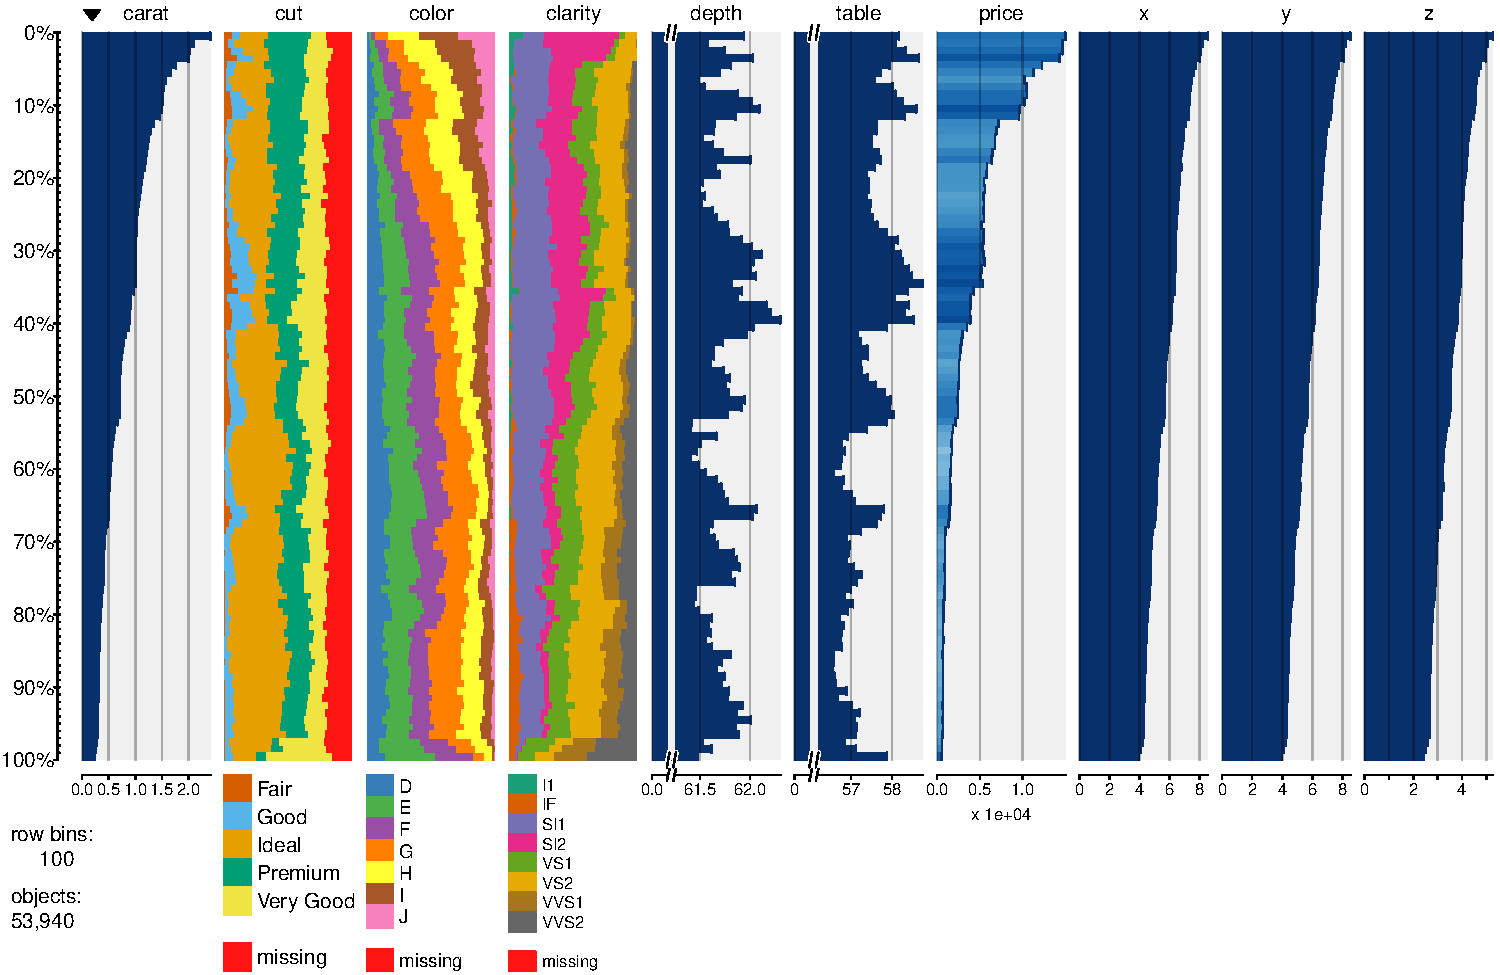
\includegraphics[width=\maxwidth]{figure/chunk2} 
\end{knitrout}

\caption{Tableplot of the diamonds dataset}
\label{fig:tp1}
\end{figure}

The result is depicted in Figure~\ref{fig:tp1}. By default, all variables of the dataset are depicted. With the argument {\tt select}, we can specify which variables are plotted. The dataset is by default sorted according to the values of the first variable. With the argument {\tt sortCol}, we can specify on which variable(s) the data is sorted.

\begin{figure}[htp]
\begin{knitrout}
\definecolor{shadecolor}{rgb}{0.969, 0.969, 0.969}\color{fgcolor}\begin{kframe}
\begin{alltt}
\hlfunctioncall{tableplot}(diamonds, select = \hlfunctioncall{c}(carat, price, cut, color, clarity), 
    sortCol = price)
\end{alltt}
\end{kframe}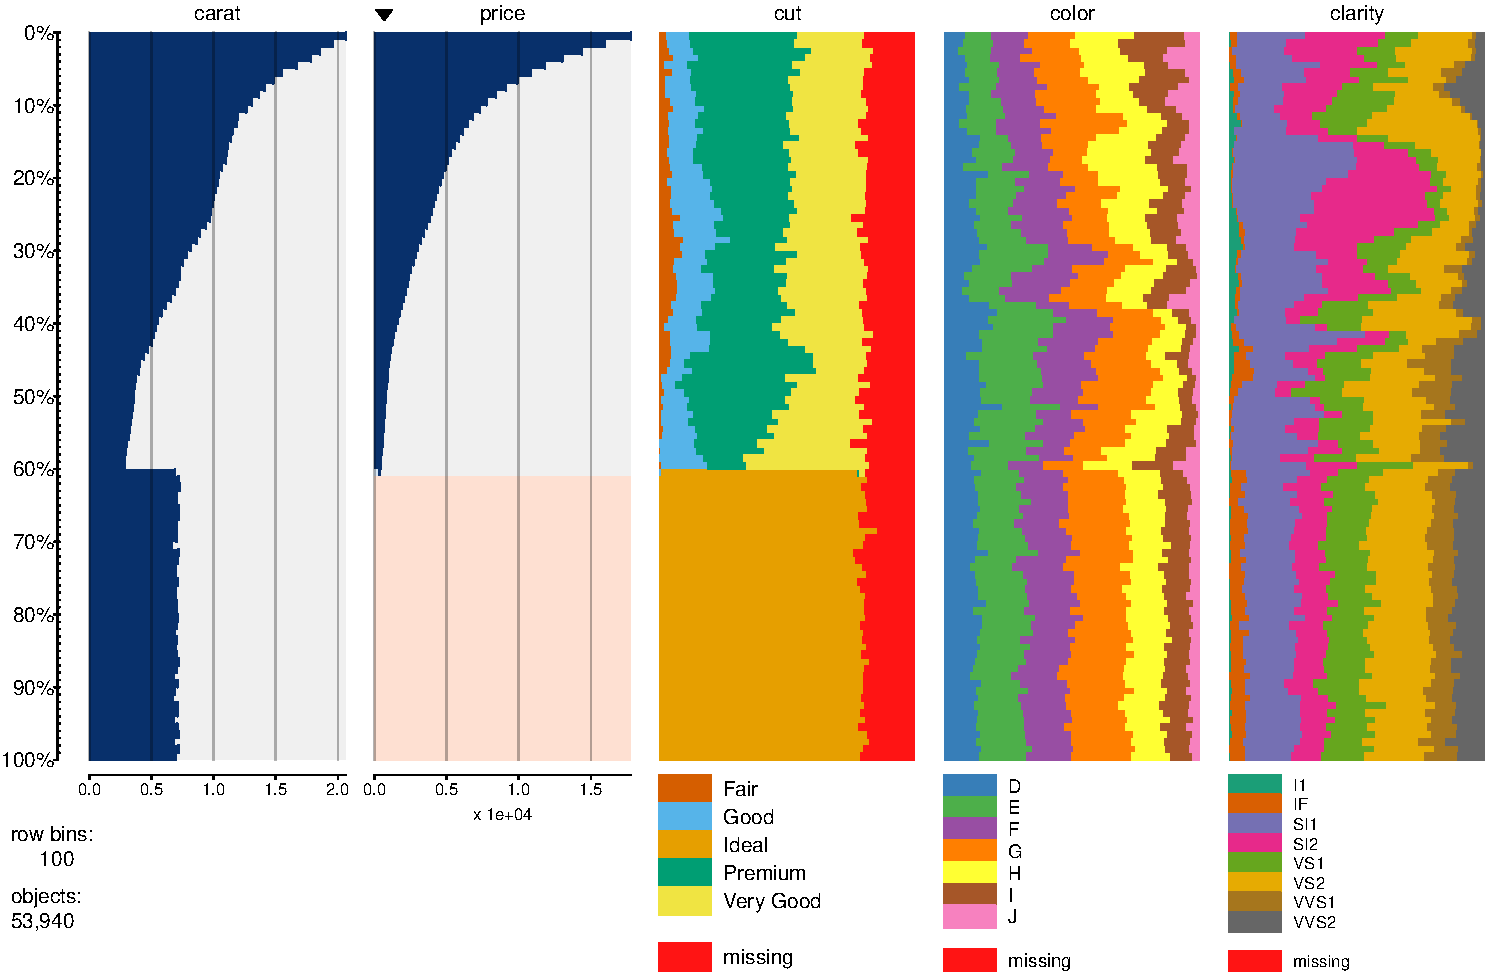
\includegraphics[width=\maxwidth]{figure/chunk3} 
\end{knitrout}

\caption{Tableplot of the diamonds dataset: sorted by price}
\label{fig:tp2}
\end{figure}

The result is illustrated in Figure~\ref{fig:tp2}. 

Setting an appropriate number of row bins (by the argument {\tt nbins}) is important, like in a histogram. A good number of row bins is a trade of between good polished but meaningless data, and detailed, but noisy data. In practice, we found that the default number of 100 usually is a good starting point.

The percentages near the vertical axis indicate which subset of the data in terms of units (rows) is depicted. The range from 0\% to 100\% in Figure~\ref{fig:tp2} means that all units of the data are plotted. 


We can focus our attention to the 5\% most expensive diamonds by setting the {\tt from} argument to 0 and the {\tt to} argument to 5:


\begin{figure}[htp]
\begin{knitrout}
\definecolor{shadecolor}{rgb}{0.969, 0.969, 0.969}\color{fgcolor}\begin{kframe}
\begin{alltt}
\hlfunctioncall{tableplot}(diamonds, select = \hlfunctioncall{c}(carat, price, cut, color, clarity), 
    sortCol = price, from = 0, to = 5)
\end{alltt}
\end{kframe}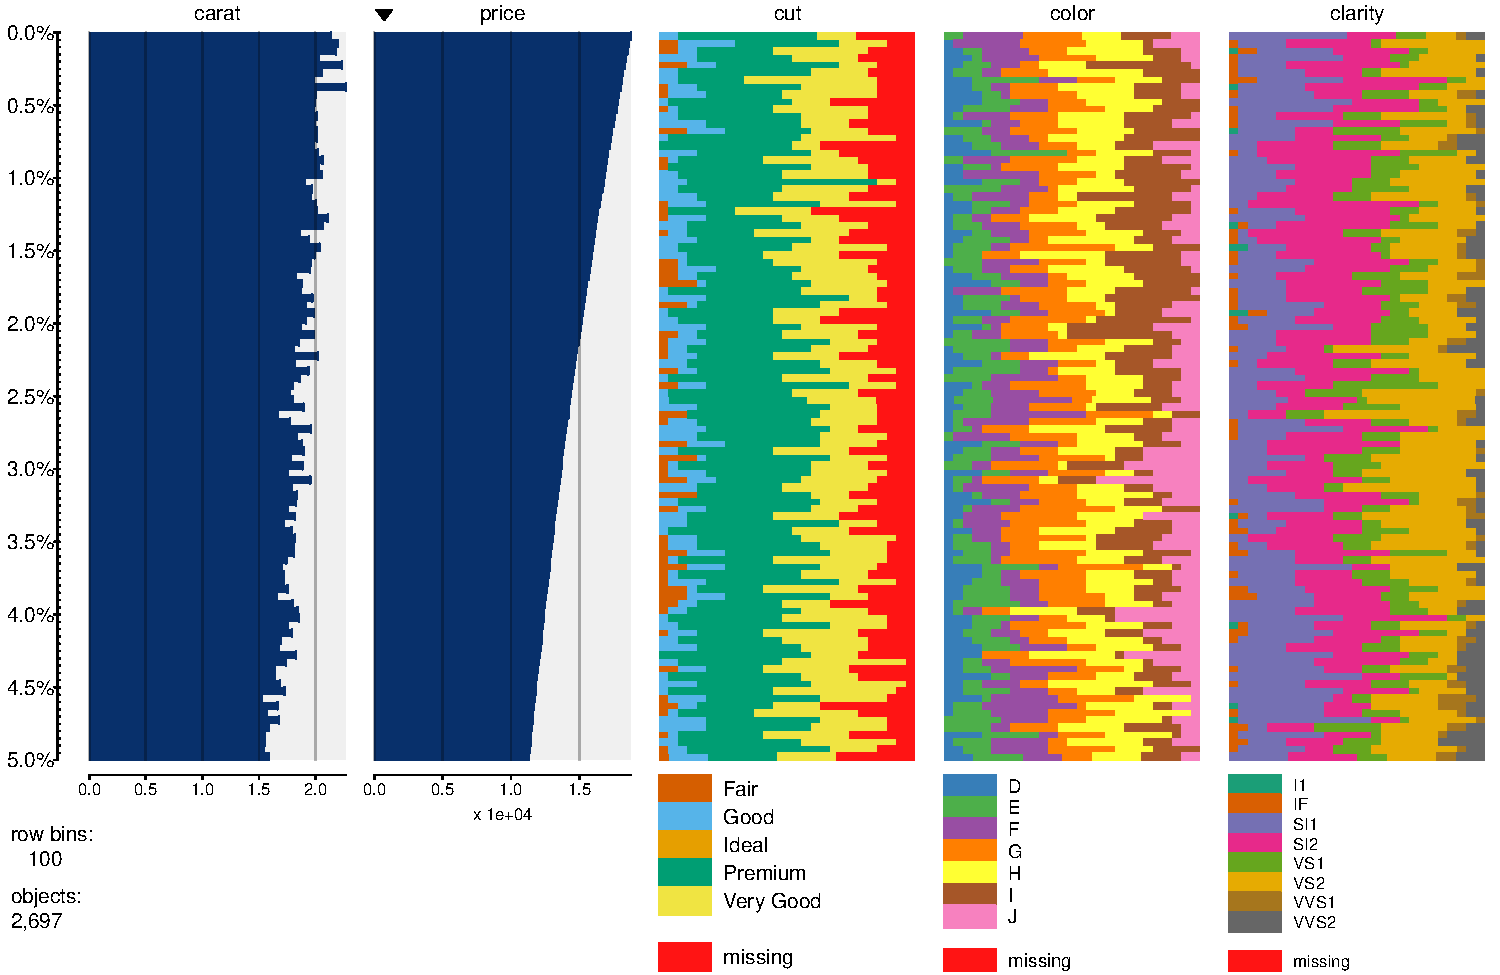
\includegraphics[width=\maxwidth]{figure/chunk4} 
\end{knitrout}

\caption{Tableplot of the diamonds dataset: zooming in}
\label{fig:tp3}
\end{figure}


Observe that in the obtained tableplot in Figure~\ref{fig:tp3}, the number of row bins is still 100, so that the number of units per row bin is now 27 instead of 540. Therefore, much more detail can be observed in this tableplot.

The vertical axis contains two sets of tick marks. The small tick marks correspond with the row bins and the large tick marks correspond with the percentages between {\tt from} and {\tt to}. The latter are determined by R's base function {\tt pretty}.


\section{Customizing the tableplot}


\subsection{Continuous variables}

For each bin of a continuous variable, the mean value is calculated (see Algorithm~\ref{alg}).
When the distribution of these mean values is exponential, it is useful to apply a logarithmic transformation. The argument {\tt scales} can be set to linear mode {\tt "lin"}, logarithmic mode {\tt "log"}, or the default value {\tt "auto"}, which automatically determines which of the former two modes is used.

Observe that the x-axes of the variables depth and table in Figure~\ref{fig:tp1} are broken. The x-axis of a variable $i$ is broken if
either
\begin{align*}
& 0 < \textit{max}(m_{i1}, m_{i2},\ldots, m_{in}) \qquad \textsc{and}\\
& \mbox{{\tt bias\_brokenX}} \cdot \textit{max}(m_{i1}, m_{i2},\ldots, m_{in}) < \textit{min}(m_{i1}, m_{i2},\ldots, m_{in}) 
\end{align*}
\textsc{or}
\begin{align*}
& 0 > \textit{min}(m_{i1}, m_{i2},\ldots, m_{in}) \qquad \textsc{and}\\
& \mbox{{\tt bias\_brokenX}} \cdot \textit{min}(m_{i1}, m_{i2},\ldots, m_{in}) > \textit{max}(m_{i1}, m_{i2},\ldots, m_{in}),
\end{align*}
where {\tt bias\_brokenX} is a bias parameter that should be a number between 0 and 1. If {\tt bias\_brokenX=1} then the above conditions are always false, which implies that the x-axes are never broken. On the other hand, if {\tt bias\_brokenX=0} then the x-axes are always broken. By default, {\tt bias\_brokenX} {\tt=0.8}, which mean that an x-axis is broken if (in case of a variable with positive values) the minimum value is at least 0.8 times the maximum value. In the diamonds dataset, this applies to the variables depth and table.


\subsection{Categorical variables}
The color palettes of categorical variables can be customized with the argument {\tt pals}. Several qualitative palettes are implemented. They can be shown by

\begin{figure}[htp]
\begin{knitrout}
\definecolor{shadecolor}{rgb}{0.969, 0.969, 0.969}\color{fgcolor}\begin{kframe}
\begin{alltt}
\hlfunctioncall{tablePalettes}()
\end{alltt}
\end{kframe}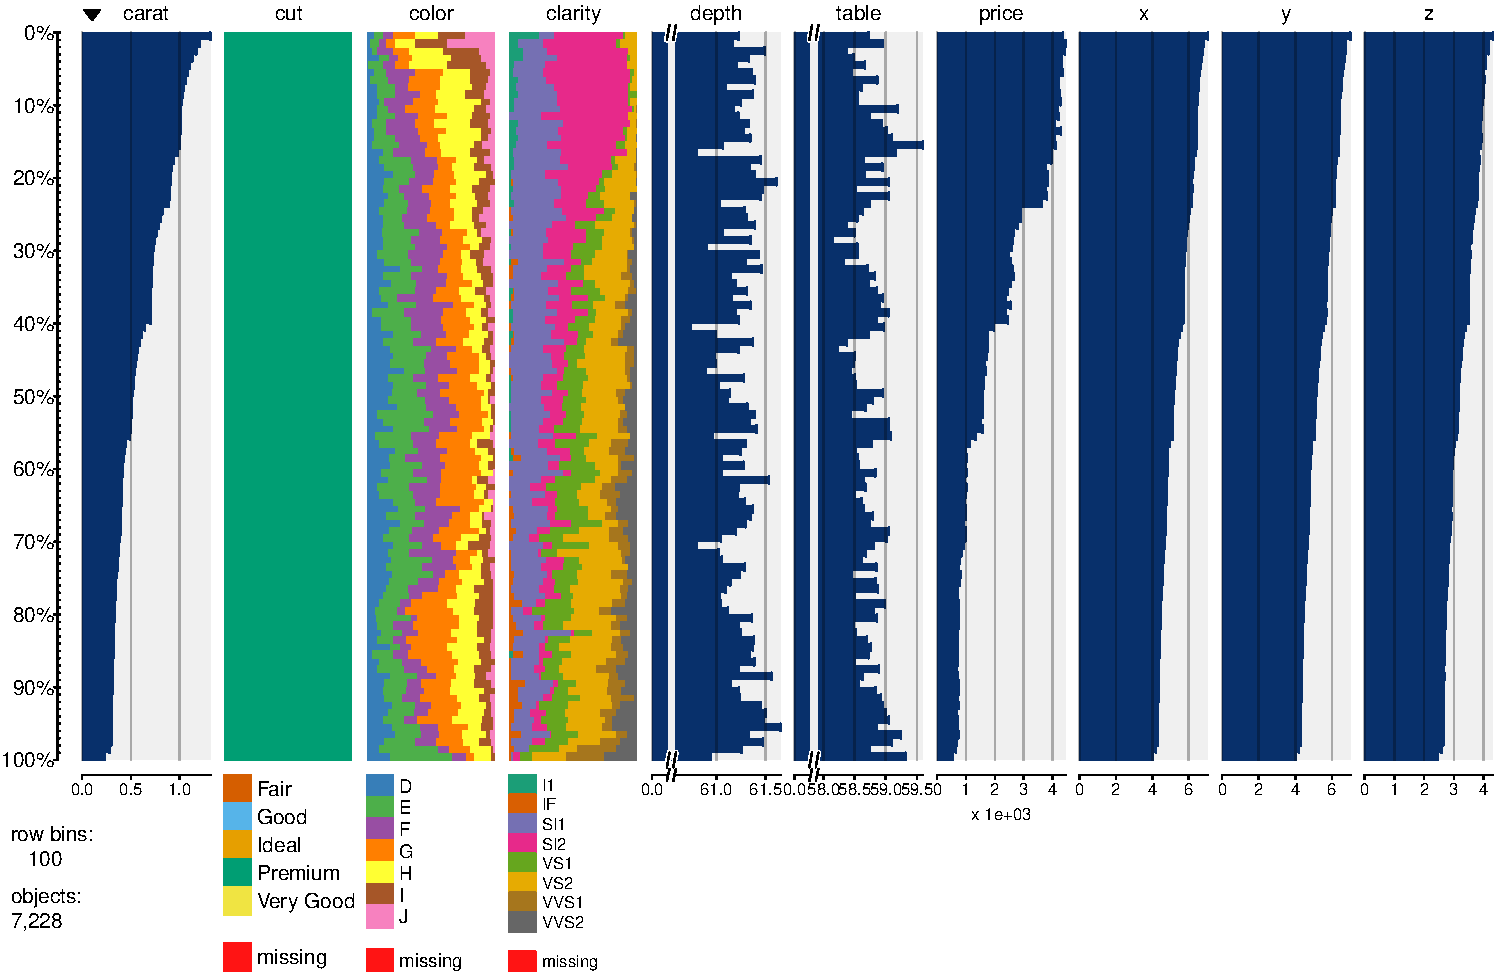
\includegraphics[width=\maxwidth]{figure/chunk5} 
\end{knitrout}

\caption{Color palettes}
\label{fig:pals}
\end{figure}

The default palette is a combination of Set1 and Set2. It has the advantage that each category has a unique color for variables with up to 16 categories.

Suppose we want a to use the default palette for the variable {\tt cut}, but starting with the seventh color, pink. Further we want the fifth palette for the variable {\tt color}, but without the first color (black), and a custom palette, say a rainbow palette, for the variable {\tt clarity}:


\begin{figure}[htp]
\begin{knitrout}
\definecolor{shadecolor}{rgb}{0.969, 0.969, 0.969}\color{fgcolor}\begin{kframe}
\begin{alltt}
\hlfunctioncall{tableplot}(diamonds, pals = \hlfunctioncall{list}(\hlstring{"\hlfunctioncall{Set1}(7)"}, \hlstring{"Set5"}, \hlfunctioncall{rainbow}(8)))
\end{alltt}
\end{kframe}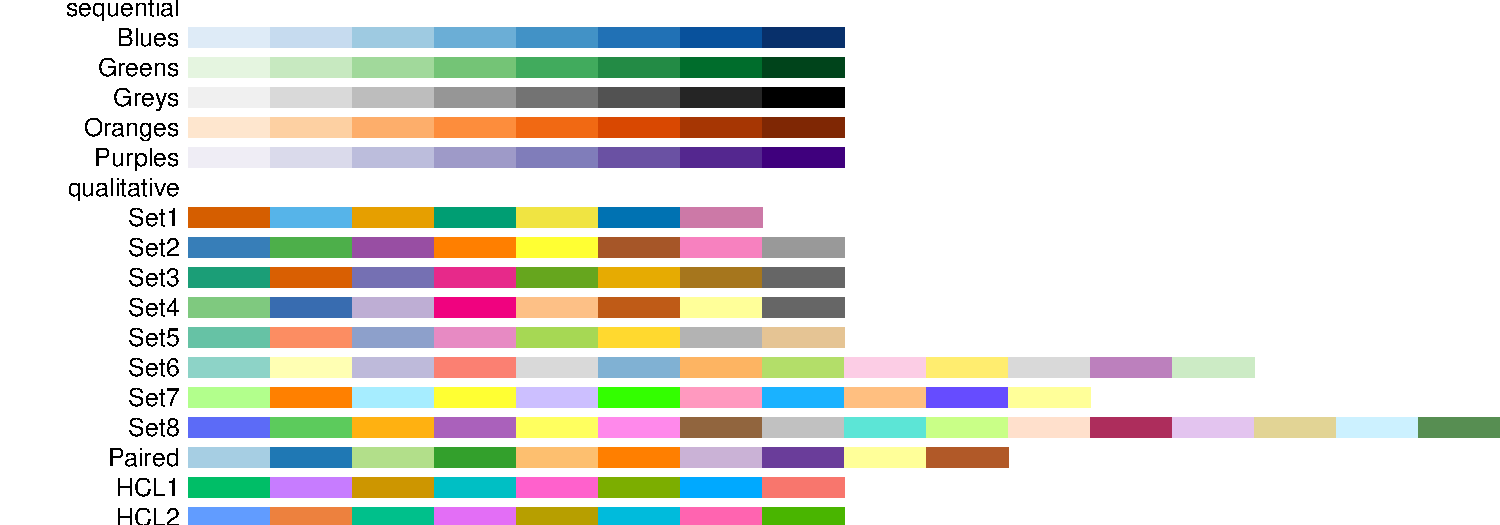
\includegraphics[width=\maxwidth]{figure/chunk6} 
\end{knitrout}

\caption{Tableplot of the diamonds dataset: other colour palettes}
\label{fig:tp4}
\end{figure}

\subsection{Filtering data}
The argument {\tt filter} serves as a filter condition for the data. The following code generates a tableplot of premium cut diamonds that cost less than 5000\$.


\begin{figure}[htp]
\begin{knitrout}
\definecolor{shadecolor}{rgb}{0.969, 0.969, 0.969}\color{fgcolor}\begin{kframe}
\begin{alltt}
\hlfunctioncall{tableplot}(diamonds, subset = price < 5000 & cut == \hlstring{"Premium"})
\end{alltt}
\end{kframe}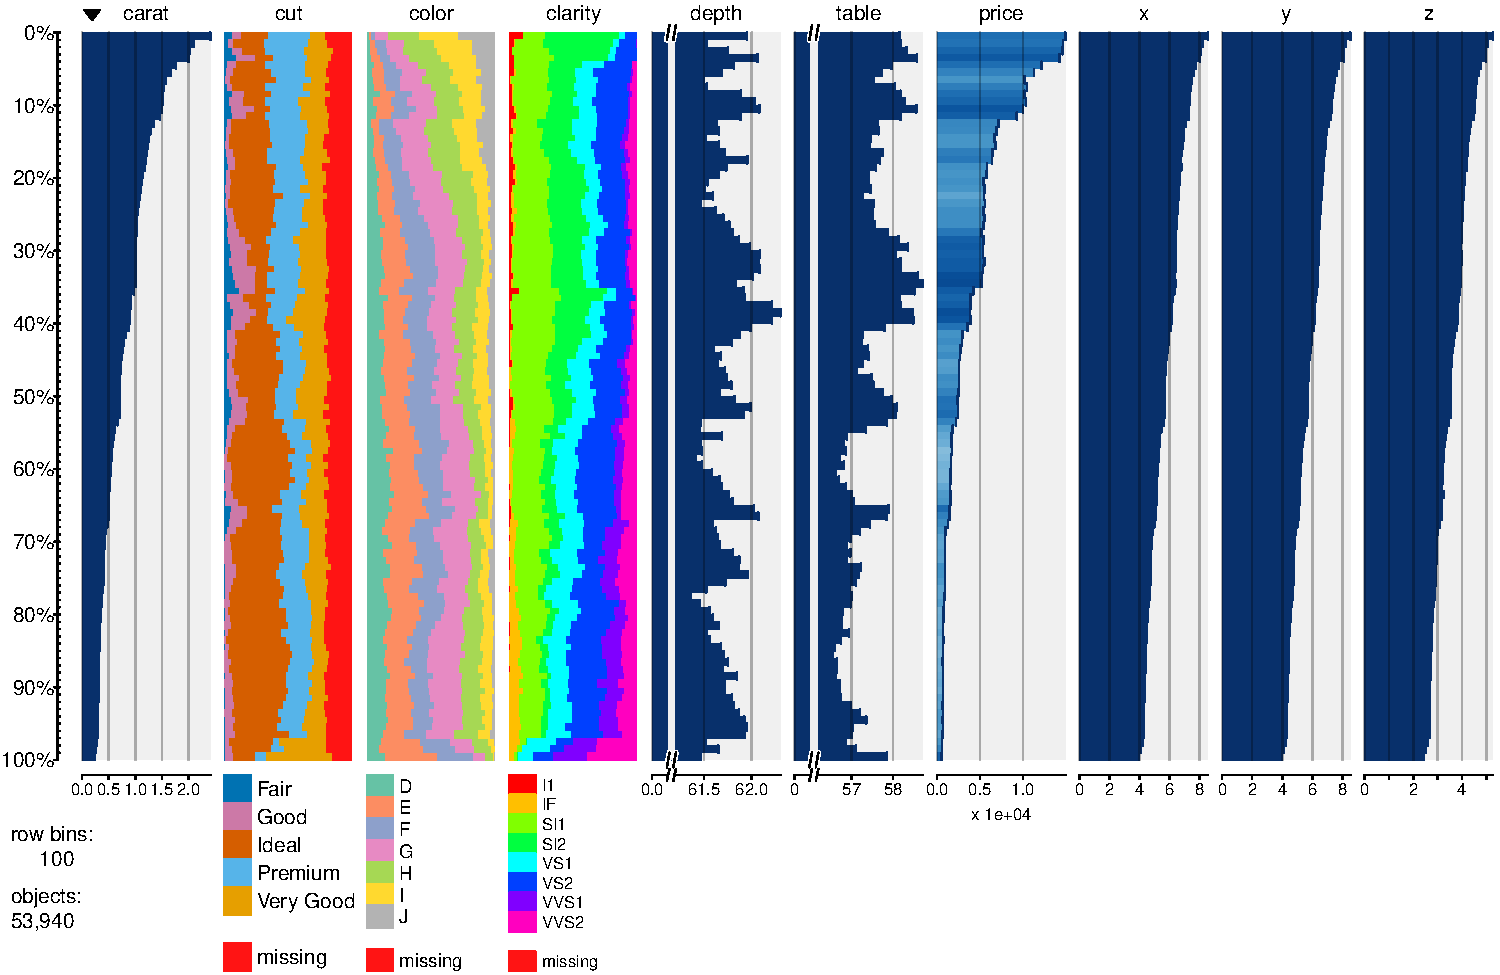
\includegraphics[width=\maxwidth]{figure/chunk7} 
\end{knitrout}

\caption{Tableplot of the diamonds dataset: filtered}
\label{fig:tp5}
\end{figure}



\subsection{The tabplot object}

The function {\tt tableplot} returns a tabplot-object, that can be used to make minor changes to the tableplot, for instance the order of columns or the color palettes. Of course, these changes can also be made by generating a new tableplot, such as in the examples above. However, if it takes considerable time to generate a tableplot, then it is practical to make minor changes immediately.

The output of the {\tt tableplot} function can be assigned to a variable. The graphical output can be omitted by setting the argument {\tt plot} to FALSE.

\begin{knitrout}
\definecolor{shadecolor}{rgb}{0.969, 0.969, 0.969}\color{fgcolor}\begin{kframe}
\begin{alltt}
tab <- \hlfunctioncall{tableplot}(diamonds, plot = FALSE)
\end{alltt}
\end{kframe}
\end{knitrout}


The tabplot-object is a list that contains all information to depict a tableplot. The generic functions {\tt summary} and {\tt plot} can be applied to the {\tt tabplot} object.

\begin{knitrout}
\definecolor{shadecolor}{rgb}{0.969, 0.969, 0.969}\color{fgcolor}\begin{kframe}
\begin{alltt}
\hlfunctioncall{summary}(tab)
\end{alltt}
\begin{verbatim}
##       general               variable1               variable2          
##  dataset  :diamonds   name       :carat        name      :cut          
##  variables:10         type       :numeric      type      :categorical  
##  objects  :53940      sort       :decreasing   sort      :NA           
##  bins     :100        scale_init :auto         categories:6            
##  from     :0%         scale_final:lin                                  
##  to       :100%                                                        
##       variable3                variable4                 variable5      
##  name      :color         name      :clarity       name       :depth    
##  type      :categorical   type      :categorical   type       :numeric  
##  sort      :NA            sort      :NA            sort       :NA       
##  categories:7             categories:8             scale_init :auto     
##                                                    scale_final:lin      
##                                                                         
##        variable6             variable7             variable8      
##  name       :table     name       :price     name       :x        
##  type       :numeric   type       :numeric   type       :numeric  
##  sort       :NA        sort       :NA        sort       :NA       
##  scale_init :auto      scale_init :auto      scale_init :auto     
##  scale_final:lin       scale_final:lin       scale_final:lin      
##                                                                   
##        variable9             variable10     
##  name       :y         name       :z        
##  type       :numeric   type       :numeric  
##  sort       :NA        sort       :NA       
##  scale_init :auto      scale_init :auto     
##  scale_final:lin       scale_final:lin      
##                                             
\end{verbatim}
\begin{alltt}
\hlfunctioncall{plot}(tab)
\end{alltt}
\end{kframe}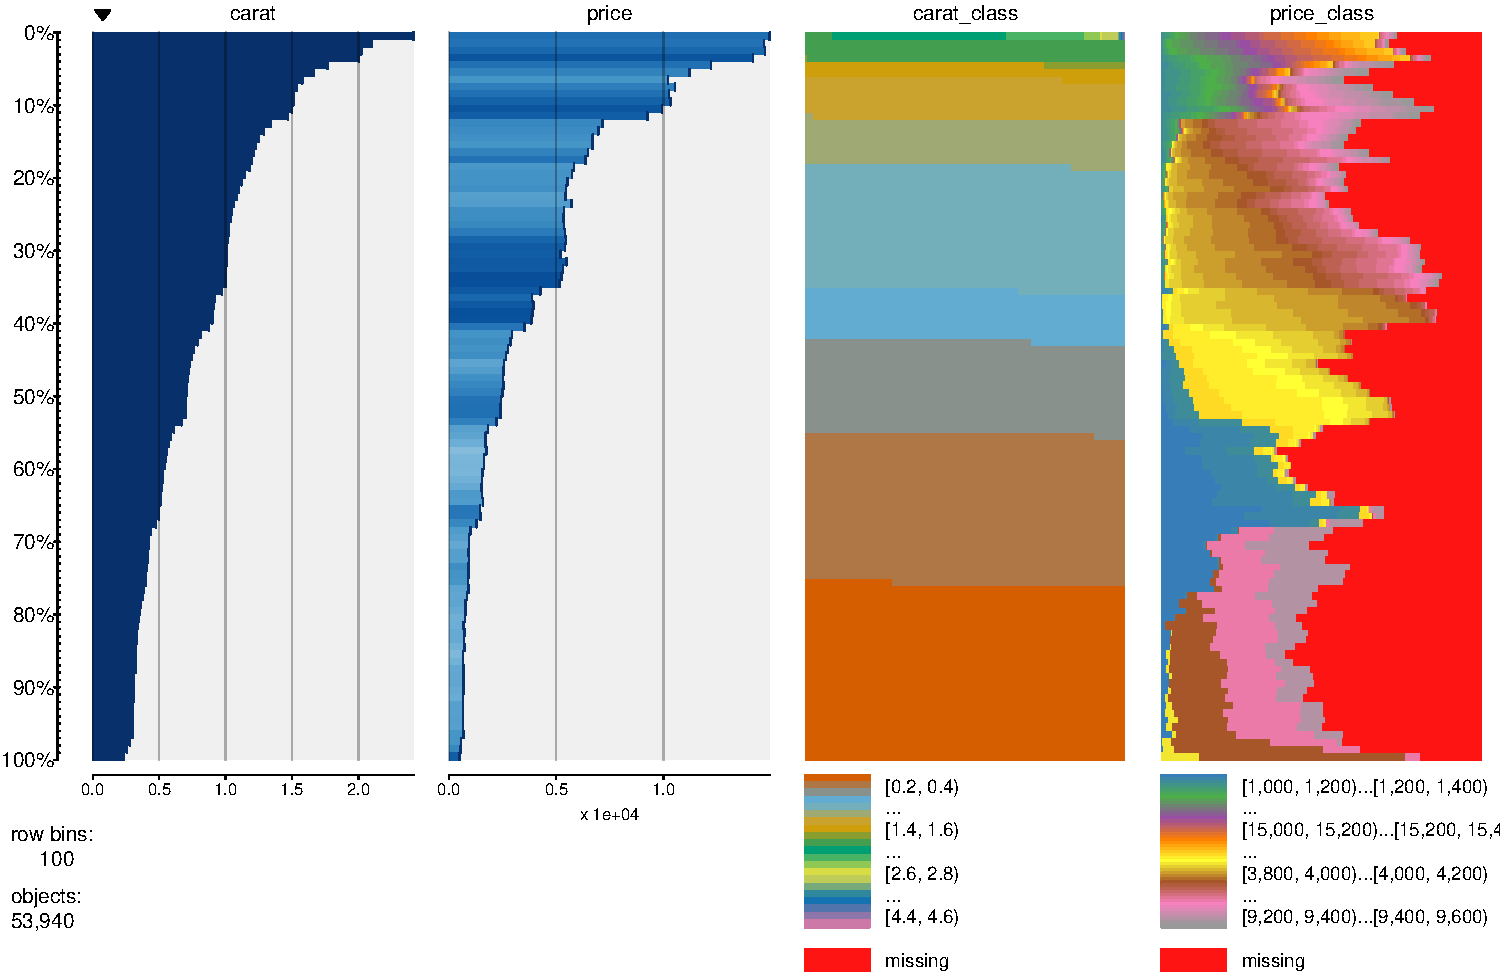
\includegraphics[width=\maxwidth]{figure/chunk9} 
\end{knitrout}


The function {\tt tableChange} is used to make minor changes to a tabplot-object. Suppose we want the columns in the order of \ref{fig:tp2}, and we want to change all color palettes to default starting with the second color.

\begin{knitrout}
\definecolor{shadecolor}{rgb}{0.969, 0.969, 0.969}\color{fgcolor}\begin{kframe}
\begin{alltt}
tab2 <- \hlfunctioncall{tableChange}(tab, colNames = \hlfunctioncall{c}(\hlstring{"carat"}, \hlstring{"price"}, \hlstring{"cut"}, \hlstring{"color"}, 
    \hlstring{"clarity"}), pals = \hlfunctioncall{list}(\hlstring{"\hlfunctioncall{Set1}(2)"}))
\hlfunctioncall{plot}(tab2)
\end{alltt}
\end{kframe}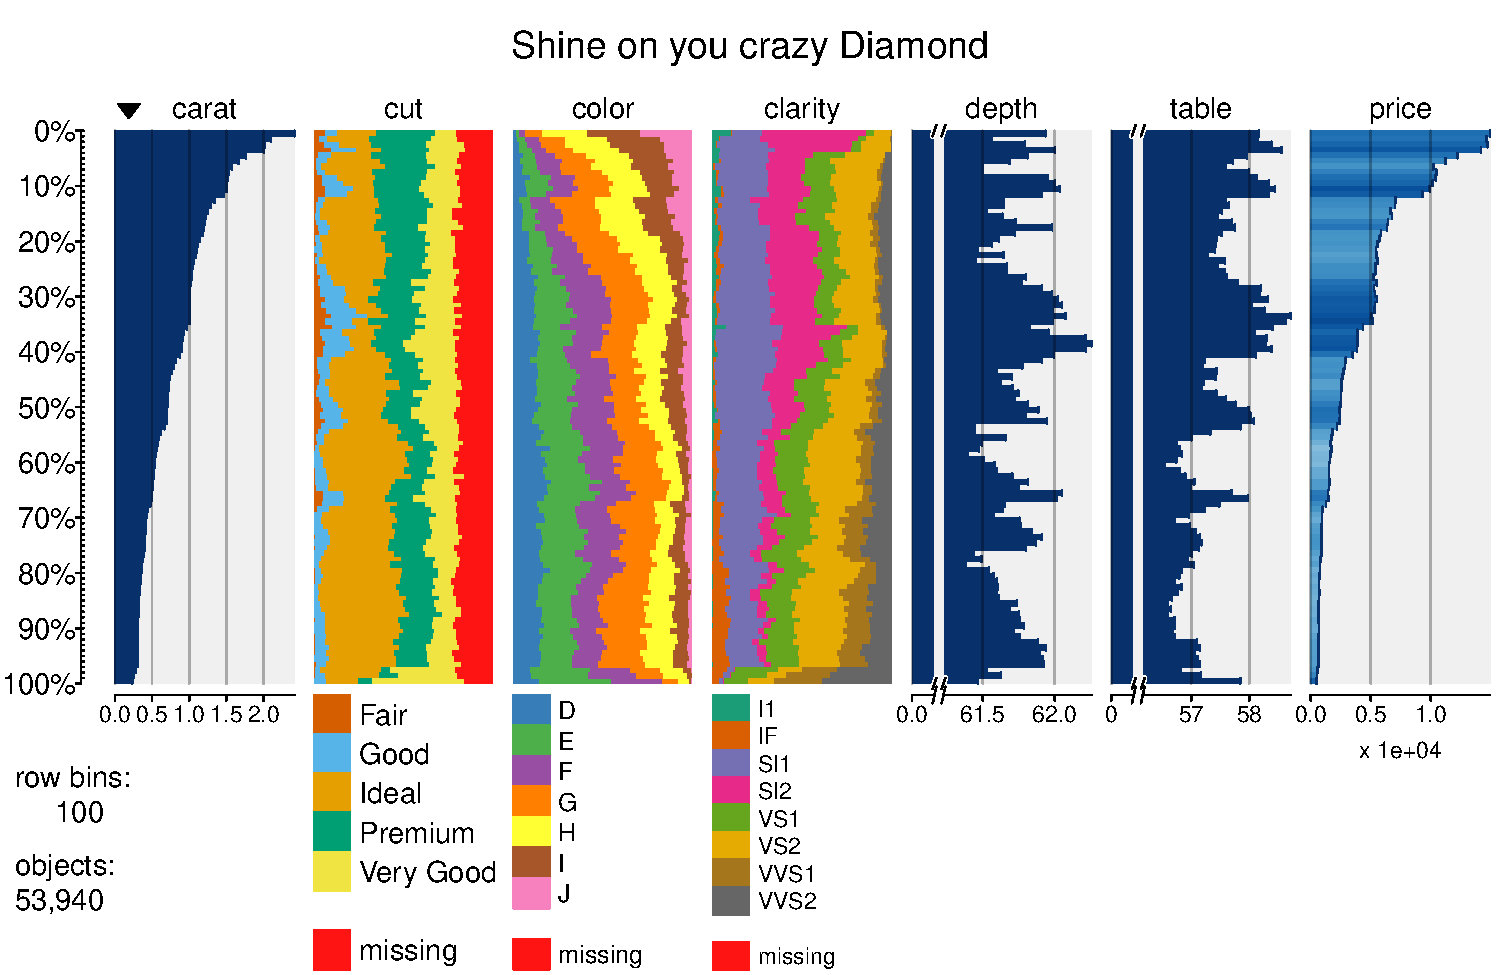
\includegraphics[width=\maxwidth]{figure/chunk10} 
\end{knitrout}


With the function {\tt tableSave}, tableplots can be saved to a desired grahical output format: pdf, eps, svg, wmf, png, jpg, bmp, or tiff.

\begin{knitrout}
\definecolor{shadecolor}{rgb}{0.969, 0.969, 0.969}\color{fgcolor}\begin{kframe}
\begin{alltt}
\hlfunctioncall{tableSave}(tab, filename = \hlstring{"diamonds.png"}, width = 5, height = 3, 
    fontsize = 6, legend.lines = 6)
\end{alltt}
\end{kframe}
\end{knitrout}





\section{Resources}
\begin{itemize}
\item Summary of the package: {\tt help(package=tabplot)}
\item The main help page: {\tt ?tabplot}
\item Project site: \url{http://code.google.com/p/tableplot/}
\item References:
\begin{itemize}
\item Tennekes, M., Jonge, E. de, Daas, P.J.H. (2011) Visual profiling of large statistical datasets. Paper presented at the 2011 New Techniques and Technologies for Statistics conference, Brussels, Belgium. (
\href{http://www.von-tijn.nl/tijn/research/publications/Tableplots.pdf}{paper}, 
\href{http://www.von-tijn.nl/tijn/research/presentations/NTTS_tableplots.pdf}{presentation}
)
\end{itemize}
\end{itemize}


\appendix
\newpage
\section{Tableplot creation algorithm}\label{secalg}
A tabplot is basically created by Algorithm~\ref{alg}.

\begin{algorithm}[h]
\caption{Create tableplot}\label{alg}
\begin{minipage}{0.8\textwidth}
\begin{algorithmic}[1]
\Require Tabular dataset $t$, column $i_s$ of which the distribution is of interest\footnote{The dataset $t$ can also be sorted according to multiple columns.}, number of row bins $n$.
\State $t'\leftarrow$ sort $t$ according to the values of column $i_s$.
\State Divide $t'$ into $n$ equally sized row bins according to the order of $t'$.
\For {each column $i$}
\If{$i$ is numeric}
\State $m_{ib}\leftarrow$ mean value per bin $b$
\State $c_{ib}\leftarrow$ fraction of missing values per bin $b$
\EndIf
\If{$i$ is categorical}
\State $\begin{aligned}[t]
		&\mbox{$f_{ijb}\leftarrow$ frequency of each category $j$ (including missing values)}\\[-3pt]
		&\mbox{per bin $b$}
	\end{aligned}$
\EndIf
\EndFor
\For {each column $i$}
\If{$i$ is numeric}
\State $\begin{aligned}[t]
		&\mbox{Plot a bar chart of the mean values $\{m_{i1}, m_{i2},\ldots, m_{in}\}$, option-}\\[-3pt]
		&\mbox{ally with a logarithmic scale. The fraction of missing values $\{c_{i1},$}\\[-3pt]
		&\mbox{$c_{i2},\ldots, c_{in}\}$ determines the lightness of the bar colour. The light-}\\[-3pt]
		&\mbox{er the colour, the more missing values occur in bin $b$. If all values}\\[-3pt]
		&\mbox{are missing, a light red bar of full length is drawn.}
	\end{aligned}$
\EndIf
\If{$i$ is categorical}
\State $\begin{aligned}[t]
		&\mbox{Plot a stacked bar chart according to the frequencies $\{f_{i1b}, f_{i2b},$}\\[-3pt]
		&\mbox{$\ldots\}$ for each bin $b$. Each category is shown is a distinct colour.}\\[-3pt]
		&\mbox{If there are missing values, they are depicted by a red colour.}
	\end{aligned}$
\EndIf
\EndFor
\Ensure Tableplot
\end{algorithmic}
\end{minipage}
\end{algorithm}




\end{document}
